\section{Clasificación automática de imágenes}

En las secciones anteriores se ha explicado las bases del aprendizaje automático y del modelo que se va a utilizar para el objetivo final de la clasificación automática de imágenes. En esta sección se detallarán los componentes principales del sistema final de clasificación adoptado.\\

Por tanto, tenemos que definir los conceptos a aprender y el conjunto de entrenamiento. Así, se describirá la base de datos ``ImageNet''\cite{imagenet_cvpr09} y la competición ILSVRC\cite{ILSVRC15}. Además, se hablará de la librería usada para el entrenamiento, Caffe \cite{jia2014caffe} y el modelo adoptado, una adaptación del modelo Alexnet\cite{NIPS2012_4824}.\\

\subsection{ImageNet e ILSVRC}

ImageNet es una base de datos de imágenes  mantenida por las universidades de Standford y Princeton. Las imágenes se organizan según la jerarquía definida en WordNet. En WordNet, cada concepto se clasifica dentro de un ``conjunto de sinónimos'' determinado, también conocido como ``synset''. ImageNet, por tanto, divide sus imágenes por synsets, teniendo según su página web 14.197.122 imágenes de 21.841 synsets diferentes. Las imágenes pasan un control de calidad y son anotadas por humanos. El objetivo es disponer de una base de datos de alta calidad, que contenga en torno a mil imágenes por concepto dentro de la jerarquía de Wordnet, que tiene en la actualidad más de 100.000 synsets.\\

El fin de esta base de datos es facilitar la tarea de la investigación en el campo de las imágenes y la visión por computador. Es claro que para poder realizar una buena investigación, se necesita una buena fuente de información. Por tanto, para poder afrontar el problema de la clasificación de imágenes a gran escala, se hace necesaria una base de datos a gran escala. Con la motivación de crear una gran base de datos para este tipo de problemas, nació ImageNet.\\

ImageNet no posee los derechos de las imágenes contenidas en la base de datos. Por ello, lo único que pueden dar de manera abierta es el enlace a la imagen, de manera similar a los buscadores de imágenes. Sin embargo, las base de datos está completamente disponible para investigadores y docentes que usen las imágenes con fines no comerciales.\\

Dentro de ImageNet, existe una competición llamada ImageNet Large Scale Visual Recognition Competition (ILSVRC). Aunque ahora la competición tiene varias modalidades distintas para competir, desde sus inicios el problema principal ha sido el de clasificar imágenes dentro de 1.000 categorías distintas. Estas categorías representan un marco muy amplio, podemos encontrar desde material de oficina como impresoras a una gran variedad de animales. Dada esta variedad tan amplia, y a ser un problema conocido, se ha tomado los datos de esta competición, en concreto la edición de 2012, para realizar el aprendizaje de nuestro modelo.\\

\subsection{Información del aprendizaje}

Para el entrenamiento del clasificador utilizamos la librería Caffe \cite{jia2014caffe}. Caffe es un framework de deep learning, desarrollado por el  Berkeley Vision and Learning Center (BVLC). Además, tiene una amplia comunidad que ayuda a mantener el código del proyecto y los modelos de acuerdo al estado del arte. Una de sus principales ventajas es la sencillez. Todas las opciones de optimización se hacen con simples cambios de configuración, sin tener que programar nada. Los modelos de redes se definen en un fichero simple, donde solamente hay que definir el tipo y la estructura de cada capa. Además, es tambíen una librería rápida, permitiendo beneficiarse del uso de tarjetas gráficas junto con las librerías CUDA y CuDNN de Nvidia.\\

\begin{figure}[H]
\begin{center}

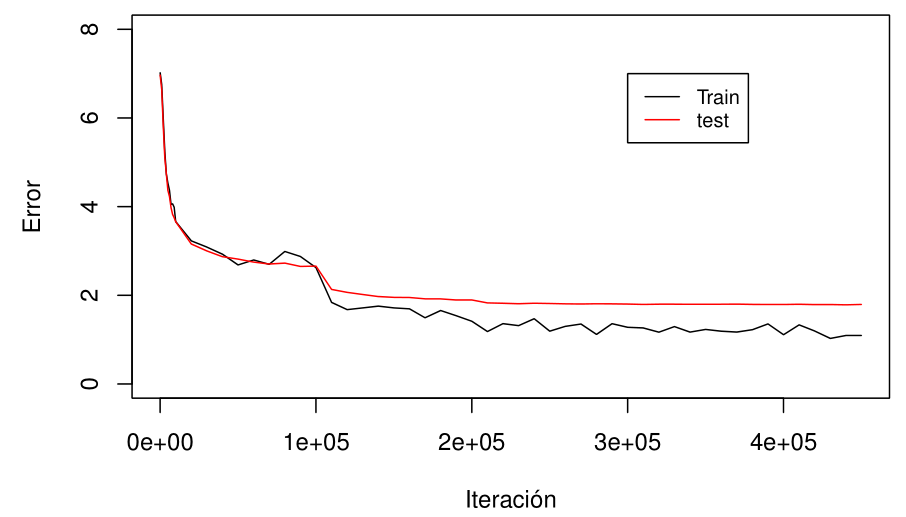
\includegraphics[width=0.9\textwidth]{img/resultados.png}
\end{center}

\caption{Resultados del entrenamiento.}
\label{resultados}
\end{figure}

El modelo entrenado fue caffenet, una versión modificada de la red Alexnet, ganadora de la competición ILSVRC en el año 2012, y que superó con creces todos los resultados de la competición, al ser la primera red en adoptar el modelo de las redes neuronales convolucionales. El entrenamiento se ejecutó sobre una gráfica GTX 1080 de Nvidia, usando las últimas versiones disponibles de las librerías CUDA y CuDNN. El proceso de aprendizaje duró más de 2 días, lastrado por bloqueos de I/O, aunque la gravedad es estos bloqueos fue menor.\\
 
En la figura \ref{resultados} podemos ver el desarrollo de los error de entrenamiento y de test de la red. Como se podría esperar, ambos errores son muy similares hasta un punto donde el error de entrenamiento empieza a bajar más que el de test. Esto empieza a mostrar signos del sobreentreno, pues muestra mejores resultados de entrenamiento que de test, cuando se esperarían resultados parecidos. Aún así, no se observa un efecto catastrófico de sobreentrenamiento. Esto puede deberse a que quizás todo el control de la dimensionalidad de las redes neuronales convolucionales consigue reducir efectivamente los problemas de sobreentrenamiento.  Los pesos seleccionados son los correspondientes a la iteración 370.000, con un error de test 1.80 y un porcentaje de acierto en la clasificación del 57.92\%.

\subsection{Ejemplos de resultados}

Vamos a ver algunos ejemplos de clasificaciones. Se muestran los cinco resultados más significativos para el clasificador, así como un indicador visual del grado de creencia de dicho resultado.\\

\begin{figure}[H]
\begin{center}

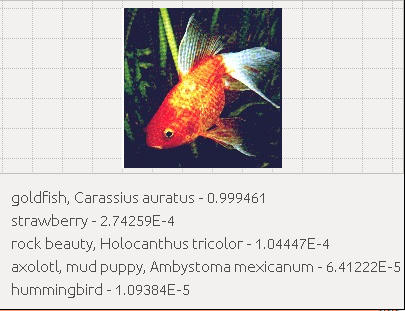
\includegraphics[width=0.6\textwidth]{img/Pez.png}
\end{center}

\caption{Resultados de clasificación de un pez .}
\end{figure}

Como ya hemos dicho tenemos un abanico de categorías muy grande. No sólo es capaz de clasificar el pez de la imagen justo en el tipo de pez que le corresponde, si no que también tenemos objetos que son mucho menos comunes.\\

\begin{figure}[H]
\begin{center}

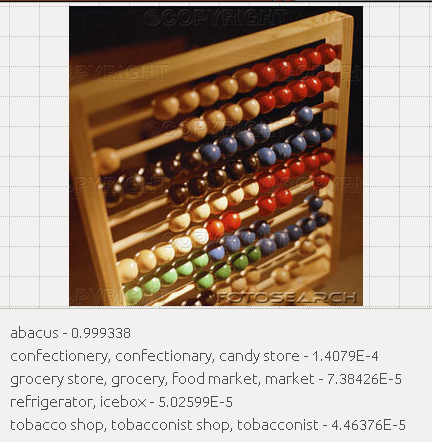
\includegraphics[width=0.5\textwidth]{img/Abaco.png}
\end{center}

\caption{Resultados de clasificación de un ábaco.}
\end{figure}

Estos resultados, dan una buena base a nuestro sistema de recuperación de imágenes. El sistema obtiene resultados muy lógicos y de una alta calidad en una gran variedad de términos lingüísticos. Pero en la siguiente imagen, vemos un pequeño inconveniente de la técnica.\\

\begin{figure}[H]
\begin{center}

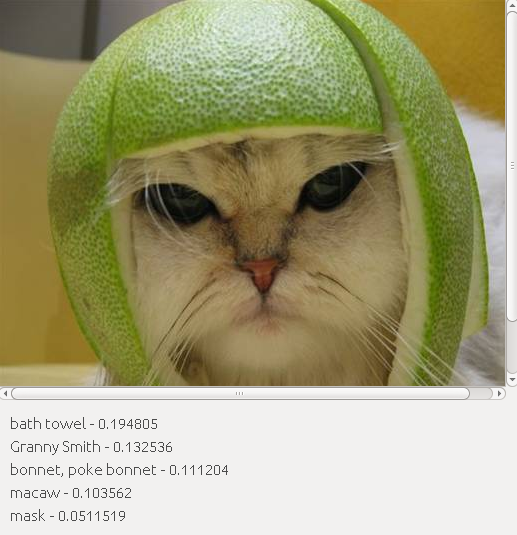
\includegraphics[width=0.5\textwidth]{img/Gatomelon.png}
\end{center}

\caption{Resultados de clasificación de un ``gato-melón''.}
\end{figure}

Al mezclar dos conceptos distintos en una sola imagen, en este caso los conceptos gato y melón, el sistema se equivoca. Esto es normal, pues se ha entrenado solo con imágenes que representan un único concepto. Aún así, este sistema se podría utilizar con este tipo de imágenes, utilizando técnicas de segmentación.\\

Por último, vemos un ejemplo de su uso para recuperar imágenes. En un conjunto de 50 imágenes variadas, al introducir la consulta ``Púa'', el sistema consigue recuperar perfectamente las 5 imágenes que encajan en esta categoría introducida.\\

\begin{figure}[H]
\begin{center}

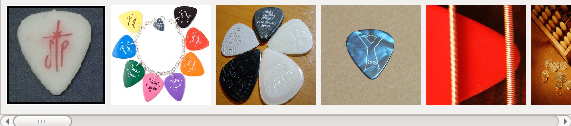
\includegraphics[width=0.9\textwidth]{img/Puas.png}
\end{center}

\caption{Recuperación de púas de guitarra.}
\end{figure}